\documentclass{beamer}
\usepackage{xeCJK}
%\usepackage{newtxtext,newtxmath}	% use Times Roman font
%\usefonttheme{serif}
\usefonttheme{professionalfonts}
%\setbeamertemplate{theorems}[numbered]
\setbeamertemplate{caption}{\insertcaption} 	% no `Figure' prefix before caption

\mode<presentation> {

%\usetheme{default}
%\usetheme{AnnArbor}
%\usetheme{Antibes}
%\usetheme{Bergen}
%\usetheme{Berkeley}
%\usetheme{Berlin}
%\usetheme{Boadilla}
%\usetheme{CambridgeUS}
%\usetheme{Copenhagen}
%\usetheme{Darmstadt}
%\usetheme{Dresden}
%\usetheme{Frankfurt}
%\usetheme{Goettingen}
%\usetheme{Hannover}
%\usetheme{Ilmenau}
%\usetheme{JuanLesPins}
%\usetheme{Luebeck}
\usetheme{Madrid}
%\usetheme{Malmoe}
%\usetheme{Marburg}
%\usetheme{Montpellier}
%\usetheme{PaloAlto}
%\usetheme{Pittsburgh}
%\usetheme{Rochester}
%\usetheme{Singapore}
%\usetheme{Szeged}
%\usetheme{Warsaw}

%\usecolortheme{albatross}
%\usecolortheme{beaver}
%\usecolortheme{beetle}
%\usecolortheme{crane}
%\usecolortheme{dolphin}
%\usecolortheme{dove}
%\usecolortheme{fly}
%\usecolortheme{lily}
%\usecolortheme{orchid}
%\usecolortheme{rose}
%\usecolortheme{seagull}
%\usecolortheme{seahorse}
%\usecolortheme{whale}
%\usecolortheme{wolverine}

%\setbeamertemplate{footline} % To remove the footer line in all slides uncomment this line
%\setbeamertemplate{footline}[page number] % To replace the footer line in all slides with a simple slide count uncomment this line
\setbeamertemplate{navigation symbols}{} % To remove the navigation symbols from the bottom of all slides uncomment this line
}

\usepackage{graphicx} % Allows including images
\usepackage{verbatim} % comments
\usepackage{tikz-cd}  % commutative diagrams
\newcommand{\tikzmark}[1]{\tikz[overlay,remember picture] \node (#1) {};}
\usepackage{booktabs} % Allows the use of \toprule, \midrule and \bottomrule in tables
\usepackage{amssymb}  % \leftrightharpoons

\newcommand{\vect}[1]{\boldsymbol{#1}}
\newcommand*\sigmoid{\vcenter{\hbox{\includegraphics{sigmoid.png}}}}

\makeatletter
\renewcommand{\boxed}[1]{\fbox{\m@th$\displaystyle\scalebox{0.9}{#1}$} \,}
\makeatother

%---------------------------- make slide margin narrower --------------------------------
%\newcommand\Wider[2][3em]{%
%	\makebox[\linewidth][c]{%
%		\begin{minipage}{\dimexpr\textwidth+#1\relax}
%			\raggedright#2
%		\end{minipage}%
%	}%
%}

%----------------------------------------------------------------------------------------
%	TITLE PAGE
%----------------------------------------------------------------------------------------

\title[Deep learning \& logic]{Combining deep learning with logical structure} % The short title appears at the bottom of every slide, the full title is only on the title page

\author{YKY 甄景贤} % Your name
\institute[] % Your institution as it will appear on the bottom of every slide, may be shorthand to save space
{
Independent researcher, Hong Kong \\ % Your institution for the title page
\medskip
\textit{generic.intelligence@gmail.com} % Your email address
}
\date{\today} % Date, can be changed to a custom date

\begin{document}

\frame{\titlepage}

\begin{frame}
\frametitle{Talk summary}
\tableofcontents
\end{frame}

%---------------- this is for when you're using \part's ----------------------------------
%\begin{frame}
%\frametitle{Summary}
%
%{\usebeamerfont*{frametitle} Part I %\usebeamercolor[fg]{frametitle}
% ~ ~ ~ Deep reinforcement learning}
%%\tableofcontents[part=1]
%
%\vspace{1.5cm}
%{\usebeamerfont*{frametitle} Part II %\usebeamercolor[fg]{frametitle}
% ~ ~ ~ Logical structure}
%%\tableofcontents[part=2]
%\end{frame}

%----------------------------------------------------------------------------------------
%	PRESENTATION SLIDES
%----------------------------------------------------------------------------------------

%------------------------------------------------
\section{Deep reinforcement learning} 

\frame{\sectionpage}

\begin{frame}
\frametitle{Problem setup}
\begin{itemize}
	\item Consider a (deep) neural network connected end-to-end to form a loop:
	\begin{equation}
	\vcenter{\hbox{\includegraphics[scale=0.5]{genifer-model-00.png}}}
	\end{equation}
	where ``deep'' means ``many layers''.
	
	\item This is referred to as a \textbf{recurrent} neural network (RNN).
\end{itemize}
\end{frame}

\begin{frame}
\frametitle{Intelligent agent}
\begin{itemize}
	\item The state vector $\vect{x}_t$ of the neural network traces out a \textbf{trajectory} in configuration space, which is analogous to a ``maze'' with \textbf{rewards} ({\color{red} $\bullet$}) inside it:
	\begin{equation}
	\vcenter{\hbox{\includegraphics[scale=0.7]{maze-trajectory.png}}}
	\end{equation}
	
	\item We regard the state $\vect{x}_t$ as the \textbf{mental state} of an intelligent agent, the rewards are given externally by a teacher to reward intelligent behavior.
\end{itemize}
\end{frame}

\begin{frame}
\frametitle{Neural network}
\begin{itemize}
	\item A neural network is a generic function with a large number of \textbf{parameters} called \textbf{weights}:
	\begin{eqnarray}
	& \mbox{\footnotesize \textbf{weight} matrix } \tikzmark{weightMatrix} \mbox{\footnotesize for each layer} \quad \quad \mbox{\footnotesize total \# of layers} \tikzmark{numLayers} \nonumber \\
	\nonumber \\
	& \vect{x}_{t+1} = \vect{F}(\vect{x}) = \sigmoid(W_1 \tikzmark{wa} \sigmoid(W_2 \tikzmark{wb} ... \sigmoid( W_L \tikzmark{wc} \tikzmark{L} \; \vect{x} )))
	\begin{tikzpicture}[overlay,remember picture]
	\draw (weightMatrix.center) +(17pt,-5pt) -- ([shift={(-10pt,10pt)}]wa.center);
	\draw (weightMatrix.center) +(21pt,-5pt) -- ([shift={(-10pt,10pt)}]wb.center);
	\draw (weightMatrix.center) +(33pt,-5pt) -- ([shift={(-10pt,10pt)}]wc.center);
	\draw (numLayers.center) +(-20pt,-5pt) -- ([shift={(-2pt,6pt)}]L.center);
	\end{tikzpicture}
	\end{eqnarray}

	\item $\sigmoid$ is the \textbf{sigmoid} function applied \textit{component-wise} to the vector $\vect{x}$:
	\begin{equation}
	\sigmoid (x) = \frac{1}{1 + e^{-x}}
	\end{equation}
	
	\item Neural networks are \textbf{universal approximators} of vector-valued functions.
\end{itemize}
\end{frame}


\begin{frame}
\frametitle{Dynamical system}
\begin{itemize}
	\item So we have a dynamical system given by the \textbf{transition function} $\vect{F}$:
	\begin{equation}
	\vect{x}_{t + 1} = \vect{F}(\vect{x}_t, \vect{u}_t)
	\end{equation}
	where $\vect{u}$ is the \textbf{control variable}.

	\item The reward at state $\vect{x}_t$ is $L(\vect{x}_t)$ which corresponds to the \textbf{Lagrangian} in the Hamiltonian formulation.  Our goal is to maximize the total reward over time:
	\begin{equation}
	\boxed{action} \quad A = \int L(\vect{x}_t) dt
	\end{equation}
	which coincides with the notion of \textbf{action} in Hamiltonian mechanics.
\end{itemize}
\end{frame}

\begin{frame}
\frametitle{background: AIXI theory}
\begin{theorem}[Hutter 2000]
The action chosen by this formula defines an \textbf{optimal} intelligent agent: \\
\begin{equation}
a_k := \arg \max_{a_k} \sum_{o_k r_k} ... \max_{a_\infty} \sum_{o_\infty r_\infty} [r_k + ... + r_\infty] \sum_{{q: U(q,a_1,...,a_\infty)}\atop{= o_1 r_1 ...o_\infty r_\infty}} 2^{-\ell(q)}
\end{equation}
$a$ction, $r$eward, $o$bservation, $U$niversal Turing Machine, $q$rogram, $k$=now
\end{theorem}
\begin{itemize}
	\item similar to my setup
	\item widely regarded by AI practitioners as ``useless'' because it involves \textbf{algorithmic} / Kolmogorov complexity.
\end{itemize}
\end{frame}

\begin{frame}
\frametitle{background: Google's DeepMind}
\begin{equation}
\vcenter{\hbox{\includegraphics[scale=0.45]{Marcus-Hutter.jpg}}}
\quad \quad
\vcenter{\hbox{\includegraphics[scale=0.3]{Juergen-Schmidhuber.jpg}}}
\nonumber
\end{equation}
\begin{center}
	\hspace{3pt} Marcus Hutter \hspace{50pt} J\"{u}ergen Schmidhuber
\end{center}
Some of their students became founding members of \textbf{DeepMind}.
\end{frame}

\begin{comment}
%------------------------------------------------

\begin{frame}
\frametitle{Blocks of Highlighted Text}
\begin{block}{Block 1}
Lorem ipsum dolor sit amet, consectetur adipiscing elit. Integer lectus nisl, ultricies in feugiat rutrum, porttitor sit amet augue. Aliquam ut tortor mauris. Sed volutpat ante purus, quis accumsan dolor.
\end{block}

\begin{block}{Block 2}
Pellentesque sed tellus purus. Class aptent taciti sociosqu ad litora torquent per conubia nostra, per inceptos himenaeos. Vestibulum quis magna at risus dictum tempor eu vitae velit.
\end{block}

\begin{block}{Block 3}
Suspendisse tincidunt sagittis gravida. Curabitur condimentum, enim sed venenatis rutrum, ipsum neque consectetur orci, sed blandit justo nisi ac lacus.
\end{block}
\end{frame}

%------------------------------------------------

\begin{frame}
\frametitle{Multiple Columns}
\begin{columns}[c] % The "c" option specifies centered vertical alignment while the "t" option is used for top vertical alignment

\column{.45\textwidth} % Left column and width
\textbf{Heading}
\begin{enumerate}
\item Statement
\item Explanation
\item Example
\end{enumerate}

\column{.5\textwidth} % Right column and width
Lorem ipsum dolor sit amet, consectetur adipiscing elit. Integer lectus nisl, ultricies in feugiat rutrum, porttitor sit amet augue. Aliquam ut tortor mauris. Sed volutpat ante purus, quis accumsan dolor.

\end{columns}
\end{frame}

\end{comment}

%------------------------------------------------
\section{Logical structure}
%------------------------------------------------

\frame{\sectionpage}

\begin{frame}
\frametitle{The world of logical structures}
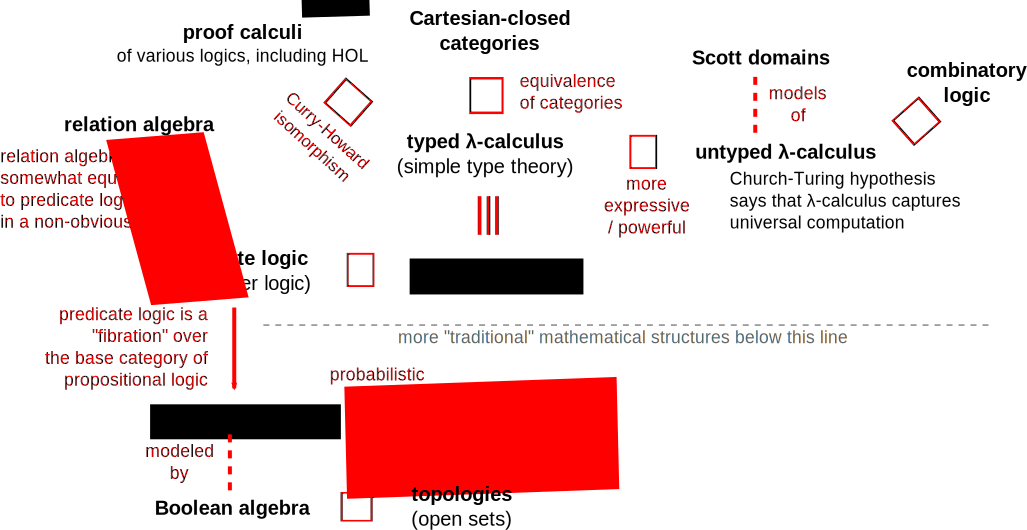
\includegraphics[scale=0.4]{world-of-logical-structures.png}
\end{frame}

\subsection{Propositional logic}

\frame{\subsectionpage}

\begin{frame}
\frametitle{Boolean lattice}
The Boolean lattice generated from 3 propositions,\\
with $2^3$ elements:
\begin{equation}
\vcenter{\hbox{\includegraphics[scale=0.4]{Boolean-lattice-eg1.png}}} \quad \cong \quad 
\vcenter{\hbox{\includegraphics[scale=0.5]{3D-cube.png}}}
\end{equation}
which is isomorphic to the \textbf{hypercube}.
\end{frame}

\begin{frame}
\frametitle{Lattice $\leftrightharpoons$ neural network}
\begin{itemize}
	\item The \textbf{output vector} of a neural network can be mapped to the \textbf{hypercube} if each output value is \textbf{binarized} to $\{0, 1\}$.  
	
	\item Each output corresponds to the \textbf{truth value} $(\top, \bot)$ of a \textbf{proposition}.  
	
	\item Thus the \textbf{Boolean lattice} is mapped to the neural network's \textbf{state vector}.
	
	\item Performing \textbf{logical deduction} would be same as traversing \textbf{vertices} of the hypercube, which is same as determining which proposition(s) become true during a deductive step.
	
	\item We may call this the ``canonical embedding'' of a Boolean lattice into a neural network's state space.
\end{itemize}
\end{frame}

\begin{frame}
\frametitle{My problem \#1}
\begin{itemize}
	\item Logic deduction is a \textbf{monotone} function going down the Boolean lattice
	\item The neural network $\vect{F}$ is ``free'' (unconstrained)
	\item Use monotonicity to constrain the \textbf{learning} algorithm of $\vect{F}$ to make it faster?
	\item Solving this problem will probably not be a major breakthrough, as neural networks are already known to handle propositional logic pretty well.
\end{itemize}
\end{frame}

\subsection{Predicate logic}

\frame{\subsectionpage}

\begin{frame}
\frametitle{Categorical logic}
\begin{columns}
	\column{0.4\textwidth}
		\begin{figure}
		\includegraphics[scale=1.0]{William-Lawvere.jpg}
		\caption{William Lawvere (1937-)}
		\end{figure}
	\column{0.6\textwidth}
		\begin{itemize}
			\item Originated the \textbf{categorical} formulation of \textbf{logic} in the 1970's.
			
			\item Established category theory as a \textbf{foundation} of mathematics similar to \textbf{set theory}.
		\end{itemize}
\end{columns}
\end{frame}

\begin{frame}
\frametitle{Predicates represented as topological open sets}
Propositional logic:
\begin{equation}
\vcenter{\hbox{\includegraphics[scale=0.4]{propositional-logic-as-topology.png}}}
\end{equation}
Predicate logic:
\begin{equation}
\vcenter{\hbox{\includegraphics[scale=0.4]{predicate-logic-as-topology.png}}}
\end{equation}
\end{frame}

\begin{frame}
\frametitle{Fibration}
\begin{equation}
\vcenter{\hbox{\includegraphics[scale=0.5]{etale-space.png}}}
\end{equation}
\end{frame}

\begin{frame}
\frametitle{Predicates as fibration}
The fibration ${\displaystyle \mathrel{\operatorname*{\downarrow}_{\mathbf{Sets}}^{\mathbf{Pred}}}}$ is a \textbf{forgetful functor}:
\begin{equation}
\vcenter{\hbox{\includegraphics[scale=0.5]{predicate-logic-as-fibration.png}}}
\label{fig:fibration}
\end{equation}
\end{frame}

\begin{frame}
\frametitle{Predicates as fibration}
\begin{itemize}
	\item The objects in $\mathbf{Pred}$ are \textit{predicates}.

	\item The objects in $\mathbf{Sets}$ are \textit{sets}, in our case there is only 1 set which is the universe.  If multiple sets, they correspond to \textbf{types} in computer science.

	\item The forgetful functor sends each predicate to its \textbf{underlying set}.
	
	\item Figure (\ref{fig:fibration}) shows 1 \textbf{fibre}.  Each fibre is a \textbf{Boolean algebra}.
\end{itemize}
\end{frame}

\begin{frame}
\frametitle{My problem \#2: the big challenge}
\begin{itemize}
	\item Use the structure of predicate logic to formulate the \textbf{learning algorithm} of neural network $\vect{F}$ so that it can perform predicate-logic deduction?
	
\end{itemize}
\end{frame}

%\cite{Jacobs1999}

\begin{frame}
\frametitle{References}
\footnotesize{
\begin{thebibliography}{99} % Beamer does not support BibTeX so references must be inserted manually as below
\bibitem[]{} Bart Jacobs (1999)
\newblock Categorical logic and type theory
% \newblock \emph{North Holland, Studies in logic} v141.

\bibitem[]{} Robert Goldblatt (2006)
\newblock Topoi -- the categorical analysis of logic

\end{thebibliography}
}
\end{frame}

\begin{frame}
\Huge{\centerline{The End}}
\end{frame}

\end{document} 